
\section*{Three y 4NT1} % Espacio para hablar del proyecto de doctorado de Emilio

\textit{THREE.studies} \citep{threestudies} hereda discusiones referentes al punto de vista, la co-presencia, el envío de información gestual a través de la web, la transmisión de flujos de audio y video a partir de servidores y el uso de fuentes sonoras en un espacio virtual. Se relaciona con \textit{4NT1} \citep{anti} y \textit{tres-estudios-abiertos} \citep{tresestudios} y forma parte de un proyecto de investigación doctoral que aborda nuevas prácticas artísticas audiovisuales en el navegador a partir de lenguajes de programación.  

\begin{figure}[H]
  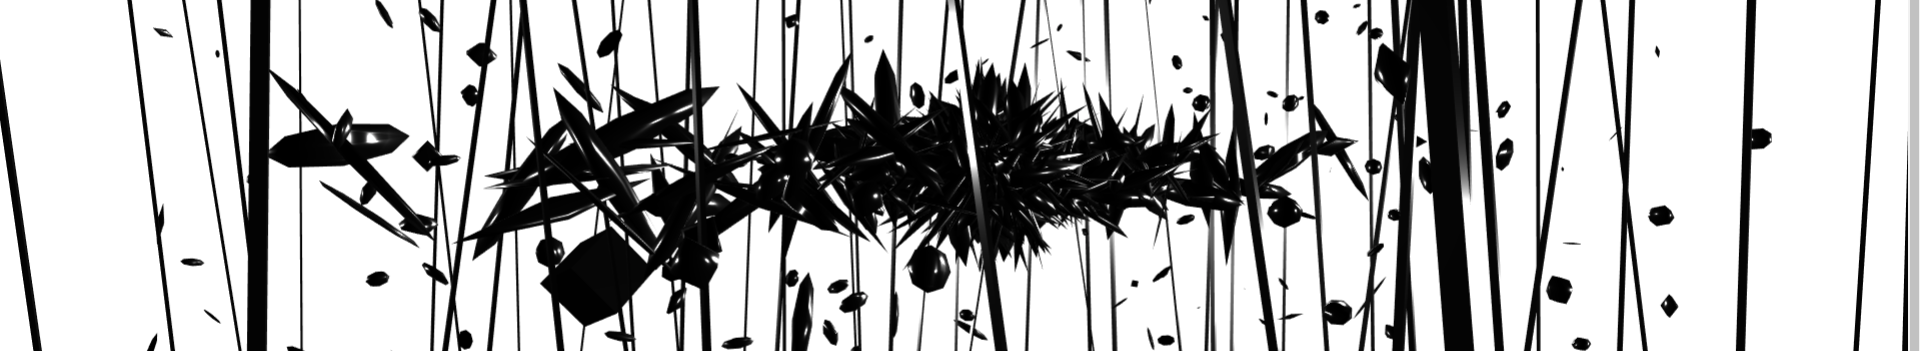
\includegraphics[width=\textwidth]{img/three.png}
  \caption{Primera iteración de THREE.studies}
\end{figure}

La primera instancia de \textit{THREE.studies}, \textit{threecln}, es un performance audiovisual para el navegador. Las señales de audio y video se encuentran en un espacio diseñado para el evento. Los elementos del escenario interactúan con las señales y proveen de retroalimentación sonora y visual al intérprete musical.

El espacio se fusiona con la interpretación y resulta en una pieza para el navegador / partitura gráfica que se transforma a sí misma cada vez que se interpreta. La obra involucra a un intérprete musical, para el caso que revisamos en este artículo, de violonchelo eléctrico, el operador de la electrónica en vivo y el equipo que mantiene la estabilidad del espacio.

El intérprete musical envía un \textit{stream} que es espacializado y que interactúa con los elementos visuales de la escena. El resultado es una obra / partitura que puede explorarse en tiempo real por el público. 

Por otro lado, \textit{4NT1} busca problematizar las relaciones que existen entre usuarios y plataformas tecnológicas; es un paso hacia la realización de usuarixs que desdibujan las fronteras de la pasividad política y económica teniendo como epicentro lo sensible. El proyecto parte de la composición visual conducida por datos. Aprovecha la investigación y el desarrollo de tres estudios abiertos, un proyecto doctoral sobre nuevas prácticas artísticas en el navegador y librerías de síntesis granular para audio y video.

La obra toma en cuenta la transformación de flujos de audio y video y se retroalimenta con la acción de agentes externos. Con técnicas de aprendizaje automático, detecta gestos faciales que son intepretados como un flujo de datos. El proyecto problematiza este flujo con el uso de tecnologías que implican una responsabilidad de los datos de usuarixs. De esta manera el proyecto pplantea una discusión que parte de la instagramización de la política y la estetización de la resistencia para desembocar en la política de la representación.

\textit{4NT1} es un pedazo de software que puede utilizarse en la vida cotidiana y que desplaza la ofuscación en el uso de tecnologías que funcionan como cajas negras al desarrollo de capas estéticas para la evasión. El proyecto contempla la comparación de dos caminos que permitan plantear una crítica al software como caja negra. Es un primer estudio de reflexión tecno-social. Retoma la idea de modularidad y se adscribe a los estudios del software, esto quiere decir que la obra se complementa con la programación, lectura, escritura y pensamiento con software.

\iffalse

- Videotitlán ?
- THREE.studies
- ¿anti? 
\fi
